\chapter{Distributed Self-Structuring Neural Network Formation Control of Multiple Coaxial UAVs With Faults}
\label{chap:formation_control}
\section{Introduction}
\label{sec:ch3_introduction}

In recent years, the use of Unmanned Aerial Vehicles (UAVs) has significantly increased across different domains due to their growing importance in civilian and military applications \cite{UAV_rev, UAV_rev1, Valavanis2015}. Consequently, researchers and industrial companies have put more interest and effort into developing these systems. This ongoing research broadly focuses on improving materials, aerodynamics, electrical components, and control strategies. The primary goal of these advancements is to ensure precise flight, smooth hovering, and, most importantly, safe operation in the presence of expected system failures \cite{Steinberg2021, Zhang2008}. Among the various available platforms, one of the most commonly used flight vehicles is the UAV with two perpendicular rotors, similar to a traditional helicopter \cite{trms_review1, Rahideh2008}. These twin-rotor architectures are highly valued for their agility and Vertical Take-Off and Landing (VTOL) capabilities, making them indispensable for executing complex operations in constrained environments \cite{trms1}.

Despite these operational advantages, controlling twin-rotor systems presents significant engineering challenges. These vehicles are characterized by complex nonlinear dynamics and exhibit strong aerodynamic cross-coupling between the main and tail rotors \cite{NonlinearCoupledDynamics1, trms2}. During real-world flights, they are constantly subjected to external wind disturbances and parametric uncertainties \cite{ExternalDisturbances1}. More importantly, their operational safety is highly vulnerable to physical faults, such as the loss of actuator effectiveness or sensor malfunctions \cite{Isermann2011, ftc_UAV_review2}. Even minor hardware failures can cause drastic trajectory deviations and lead to severe system instability if they are not compensated for quickly and effectively \cite{Steinberg2021}.

To address these challenges, various control strategies have been proposed in the literature. Many studies use classical control techniques like Proportional-Integral-Derivative (PID) controllers or conventional nonlinear methods \cite{PID1, lqr1, Backstepping_Ref}. However, these approaches still depend heavily on accurate mathematical models and struggle when facing severe uncertainties. To overcome this, recent works have combined intelligent tools like Fuzzy Logic Systems (FLS) or Neural Networks (NN) to estimate unknown nonlinearities, alongside Fault-Tolerant Control (FTC) methods to handle failures \cite{rbfnn2, NN_Control_Ref, ftc1}. Despite these improvements, traditional controllers typically guarantee only asymptotic or finite-time convergence. This means their recovery time depends heavily on the initial state of the system when a fault occurs \cite{Bhat2000}. In the event of an unexpected fault, an indispensable need remains for fast conversions. There is an urgent requirement for fast fault compensation and tracking convergence within a strict, pre-calculated short period of time, completely independent of the initial conditions \cite{fxt, Zuo2018}.

That is why we propose our controller in this chapter to address this specific gap: a Fixed-Time Fault-Tolerant Adaptive Neural Network Controller \cite{my1article, Bacha2024}. This proposed strategy relies on the backstepping technique enhanced with fixed-time stability. It uses Radial Basis Function Neural Networks (RBFNN) to online estimate and compensate for lumped uncertainties, external disturbances, and faults \cite{Park1991, rbfnn1}. Furthermore, it utilizes a metaheuristic optimization algorithm, specifically the Grey Wolf Optimizer (GWO), to optimally tune the controller parameters, balancing tracking precision with a smooth control effort \cite{gwo, glida_thesis}. To validate this controller, we use the Twin Rotor Multiple Input Multiple Output System (TRMS) as our experimental platform. The TRMS dynamics resemble a complex helicopter, making it a highly challenging and ideal grounded prototype to test advanced fault-tolerant control strategies \cite{Juang2005, trms4}.

The main contributions of this chapter provide a comprehensive solution to the twin-rotor control problem. This work ensures the fixed-time stability and precise trajectory tracking of the system despite severe actuator and sensor faults, structural uncertainties, and external disturbances. Additionally, the integration of the GWO algorithm successfully eliminates the need for manual parameter tuning. This optimization not only guarantees theoretical convergence but also prevents excessive mechanical wear on the actuators by enforcing smooth and bounded control signals.

The remainder of this chapter is organized as follows. Section \ref{sec:trms_modeling} presents the mathematical modeling of the TRMS, including the formulation of the sensor and actuator faults. Section \ref{sec:trms_control_design} details the design of the fixed-time neural network controller and provides the rigorous stability analysis. The optimization setup using the GWO is discussed in Section \ref{sec:trms_optimization}. Finally, Section \ref{sec:trms_results} provides the simulation results to validate the proposed approach, followed by a conclusion in Section \ref{sec:trms_conclusion}.
\section{Introduction}
\label{sec:formation_intro}

The successful application of single Unmanned Aerial Vehicles (UAVs) has naturally led to the next frontier in autonomous systems: the cooperative control of multi-UAV teams. A formation of multiple UAVs, or a "swarm," can perform complex tasks more efficiently, robustly, and flexibly than a single, highly sophisticated vehicle. Applications such as collaborative reconnaissance, large-area search and rescue, and coordinated payload transport are uniquely enabled by the ability of multiple agents to fly in a prescribed geometric pattern.

Despite these advantages, coordinating the flight of multiple UAVs introduces significant challenges. The controller for each UAV must not only manage its own complex dynamics but also maintain its position and orientation relative to its neighbors, often under conditions of limited communication and environmental uncertainty. Moreover, the overall reliability of the formation depends on the health of every individual agent. A single fault—whether in an actuator or a sensor—can compromise the stability of the entire group if not handled properly.

This chapter addresses these challenges by presenting a distributed fixed-time fault-tolerant formation control strategy for a swarm of coaxial rotor UAVs. The proposed approach builds on the theoretical foundations of fixed-time stability and self-structuring neural networks established in the preceding chapters. Specifically, a distributed control architecture is introduced in which each UAV relies only on information from its immediate neighbors, enhancing scalability and robustness against communication changes. To ensure rapid and predictable convergence to the desired formation, even in the presence of large initial errors, a fixed-time sliding mode control technique is designed for both the position and attitude dynamics of each UAV. Furthermore, the control scheme is explicitly constructed to tolerate faults in both actuators and sensors, thereby guaranteeing that the stability of the formation is preserved even when individual agents experience failures.

The stability of the proposed distributed control framework is rigorously established using Lyapunov theory, and its effectiveness is validated through extensive numerical simulations conducted under various fault conditions and switching communication topologies.

\section{Description of Communication Network}
\label{sec:communication_network}

The interaction and information exchange between the $N$ UAVs in the formation is modeled using graph theory. The communication topology can be represented by a time-varying, undirected graph $\mathcal{G}(t) = (\mathcal{V}, \mathcal{E}(t))$, where $\mathcal{V} = \{1, 2, \dots, N\}$ is the set of nodes (UAVs) and $\mathcal{E}(t) \subseteq \mathcal{V} \times \mathcal{V}$ is the set of edges representing communication links at time $t$. An edge $(i, j) \in \mathcal{E}(t)$ exists if UAV $i$ and UAV $j$ can exchange information.

The structure of the graph is described by the adjacency matrix $\mathbf{A}(t) = [a_{ij}(t)] \in \mathbb{R}^{N \times N}$, where $a_{ij}(t) > 0$ if $(j, i) \in \mathcal{E}(t)$, and $a_{ij}(t) = 0$ otherwise. The Laplacian matrix, $\mathbf{L}(t) = [l_{ij}(t)] \in \mathbb{R}^{N \times N}$, is defined as $l_{ii}(t) = \sum_{j=1, j \neq i}^{N} a_{ij}(t)$ and $l_{ij}(t) = -a_{ij}(t)$ for $i \neq j$.

A virtual leader, indexed by 0, provides the reference trajectory for the formation. The communication link between the virtual leader and the follower UAVs is described by a diagonal matrix $\mathbf{B}(t) = \text{diag}\{b_1(t), \dots, b_N(t)\}$, where $b_i(t) > 0$ if UAV $i$ can receive information from the leader, and $b_i(t) = 0$ otherwise. It is assumed that the graph is connected and at least one follower is connected to the virtual leader at all times.

\begin{figure}[h!]
  \centering
  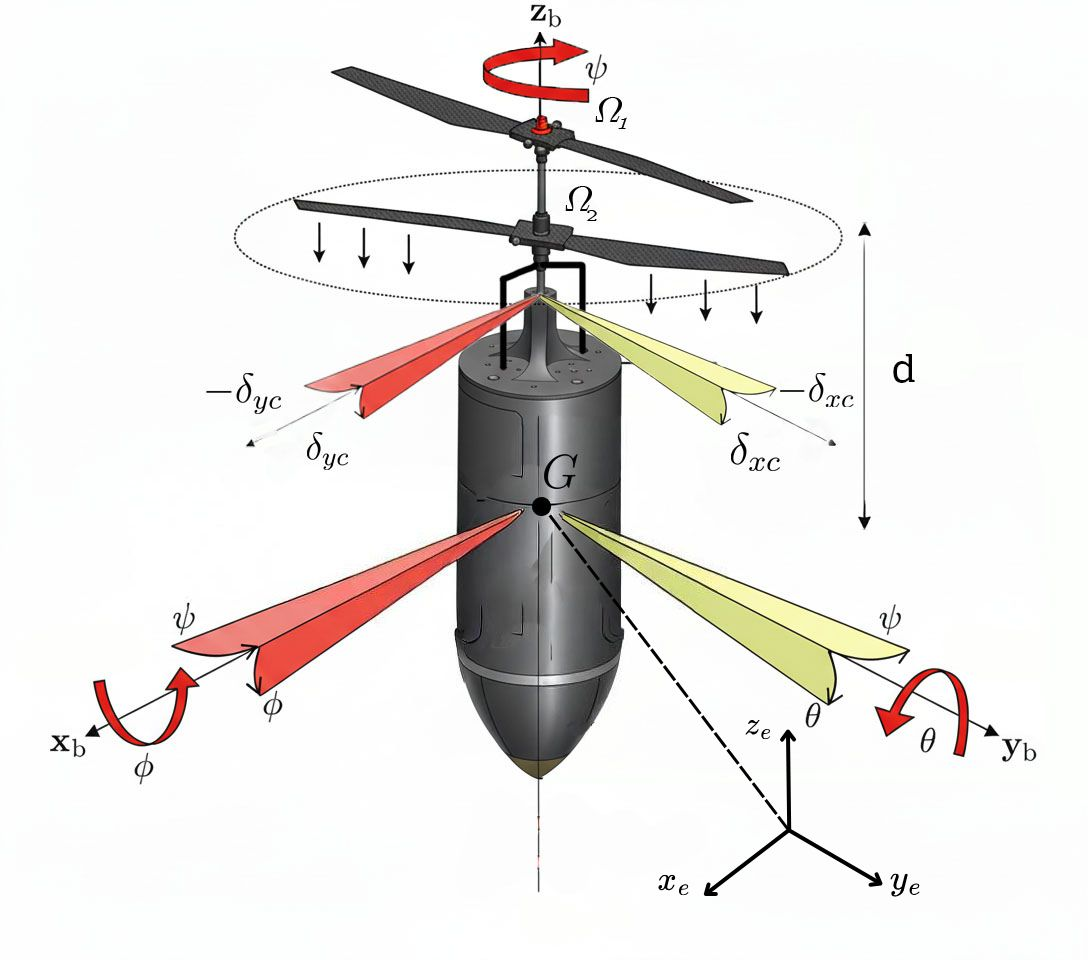
\includegraphics[width=0.6\textwidth]{Thesis_ICD/figure5/coaxial.jpg}
  \caption{Coaxial rotor vehicle configuration.}
  \label{fig:coaxial_configuration}
\end{figure}

\section{Coaxial Dynamic Model}
\label{sec:coaxial_dynamics}

The coaxial rotor UAV is an underactuated aerial vehicle with six degrees of freedom (6-DOF). Its dynamics are strongly nonlinear due to the coupling between translational and rotational motions, the counter-rotating coaxial rotors, and the swashplate mechanisms that regulate blade incidence angles. In this section, we provide a detailed derivation of the mathematical model of the coaxial UAV, which will be used for control design and stability analysis.

Two coordinate frames are introduced: the inertial (Earth-fixed) frame $\mathcal{E}(o_e,x_e,y_e,z_e)$ and the body-fixed frame $\mathcal{B}(o_b,x_b,y_b,z_b)$, whose origin is located at the center of gravity of the UAV. The UAV position in the inertial frame is denoted by $P = [x,y,z]^T$, while its orientation is described by the Euler angles $\eta = [\phi, \theta, \psi]^T$, where $\phi$, $\theta$, and $\psi$ represent roll, pitch, and yaw angles, respectively.

The transformation between the body and inertial frames is given by the rotation matrix
\begin{equation}
R =
\begin{bmatrix}
c_\theta c_\psi & s_\phi s_\theta c_\psi - c_\phi s_\psi & c_\phi s_\theta c_\psi + s_\phi s_\psi \\
c_\theta s_\psi & s_\phi s_\theta s_\psi + c_\phi c_\psi & c_\phi s_\theta s_\psi - s_\phi c_\psi \\
-s_\theta       & s_\phi c_\theta                         & c_\phi c_\theta
\end{bmatrix},
\end{equation}
where $s(\cdot)$ and $c(\cdot)$ denote sine and cosine functions.

Applying Newton–Euler dynamics, the translational and rotational motions are expressed as
\begin{align}
m\ddot{P} &= RT - mg
\begin{bmatrix}
0 \\ 0 \\ 1
\end{bmatrix}
+ F_{ext}, \\
J\ddot{\eta} &= \Psi_\eta \tau - C(\eta,\dot{\eta})\dot{\eta} + \tau_{ext},
\end{align}
where $m$ is the mass, $J = \text{diag}(I_x,I_y,I_z)$ the inertia matrix, $F_{ext}$ and $\tau_{ext}$ represent external forces and torques, and $C(\eta,\dot{\eta})$ denotes Coriolis and gyroscopic effects. The matrix $\Psi_\eta$ relates Euler angle rates to angular velocities.

The coaxial UAV employs two rotors with angular velocities $\Omega_1$ (upper rotor) and $\Omega_2$ (lower rotor). The swashplate deflections $\delta_{cx}, \delta_{cy}$ regulate the cyclic pitch of the lower rotor. The generated thrust vector can be expressed as
\begin{equation}
T =
\begin{bmatrix}
T_x \\ T_y \\ T_z
\end{bmatrix}
=
\begin{bmatrix}
- k_\beta \sin \delta_{cy} \cos \delta_{cx} \, \Omega_2^2 \\
- k_\beta \sin \delta_{cx} \, \Omega_2^2 \\
k_\alpha \Omega_1^2 + k_\beta \cos \delta_{cx} \cos \delta_{cy} \, \Omega_2^2
\end{bmatrix},
\end{equation}
where $k_\alpha$ and $k_\beta$ are aerodynamic thrust coefficients.

The corresponding control torques are given by
\begin{equation}
\tau =
\begin{bmatrix}
\tau_\phi \\ \tau_\theta \\ \tau_\psi
\end{bmatrix}
=
\begin{bmatrix}
- d k_\beta \sin \delta_{cx} \, \Omega_2^2 \\
d k_\beta \sin \delta_{cy} \cos \delta_{cx} \, \Omega_2^2 \\
\gamma_1 \Omega_1^2 - \gamma_2 \Omega_2^2
\end{bmatrix},
\end{equation}
where $d$ is the distance between the center of gravity and the rotor hub, and $\gamma_1,\gamma_2$ are aerodynamic yaw control coefficients.

For small cyclic angles $\delta_{cx}, \delta_{cy}$, we use the approximations $\cos \delta_{cx} \approx \cos \delta_{cy} \approx 1$, $\sin \delta_{cx} \approx \delta_{cx}$, and $\sin \delta_{cy} \approx \delta_{cy}$. Under these conditions, the translational and rotational dynamics simplify to
\begin{align}
\ddot{x} &= \frac{1}{m} \big( (\cos \phi \sin \theta \cos \psi + \sin \phi \sin \psi) (k_\alpha \Omega_1^2 + k_\beta \Omega_2^2) \big), \\
\ddot{y} &= \frac{1}{m} \big( (\cos \phi \sin \theta \sin \psi - \sin \phi \cos \psi) (k_\alpha \Omega_1^2 + k_\beta \Omega_2^2) \big), \\
\ddot{z} &= \frac{1}{m} \big( (\cos \phi \cos \theta)(k_\alpha \Omega_1^2 + k_\beta \Omega_2^2) \big) - g, \\
\ddot{\phi} &= \frac{I_y - I_z}{I_x}\dot{\theta}\dot{\psi} - \frac{d k_\beta}{I_x} \, \delta_{cx}\Omega_2^2, \\
\ddot{\theta} &= \frac{I_z - I_x}{I_y}\dot{\phi}\dot{\psi} + \frac{d k_\beta}{I_y} \, \delta_{cy}\Omega_2^2, \\
\ddot{\psi} &= \frac{I_x - I_y}{I_z}\dot{\phi}\dot{\theta} + \frac{1}{I_z} (\gamma_1 \Omega_1^2 - \gamma_2 \Omega_2^2).
\end{align}

The control variables $\Omega_1, \Omega_2, \delta_{cx}, \delta_{cy}$ can be mapped to the virtual control inputs $T_z$, $\tau_\phi$, $\tau_\theta$, and $\tau_\psi$. In particular, one has
\begin{align}
\Omega_1^2 &= \frac{\gamma_2 T_z - k_\beta \tau_\psi}{k_\alpha \gamma_2 + k_\beta \gamma_1}, \\
\Omega_2^2 &= \frac{\gamma_1 T_z - k_\alpha \tau_\psi}{k_\alpha \gamma_2 + k_\beta \gamma_1}, \\
\delta_{cx} &= -\frac{\tau_\phi}{d k_\beta \Omega_2^2}, \qquad
\delta_{cy} = \frac{\tau_\theta}{d k_\beta \Omega_2^2}.
\end{align}

In practical applications, actuator and sensor faults may occur and can significantly deteriorate the performance of the UAV. Actuator faults are modeled as multiplicative and additive uncertainties affecting the commanded control inputs. For the $i$-th actuator, the faulty signal is represented as
\begin{equation}
u_{a,i}(t) = \rho_i(t) u_i(t) + \zeta_i(t),
\end{equation}
where $u_i(t)$ is the nominal control input, $\rho_i(t) \in [\underline{\rho},1]$ describes partial loss of effectiveness, and $\zeta_i(t)$ represents an unknown bias fault.

Sensor faults are considered in the measurements of the translational velocity $\dot{P}$ and angular velocity $\dot{\eta}$. The faulty sensor outputs are modeled as
\begin{equation}
\dot{P}_m(t) = \dot{P}(t) + f_v(t), \qquad \dot{\eta}_m(t) = \dot{\eta}(t) + f_\omega(t),
\end{equation}
where $f_v(t)$ and $f_\omega(t)$ denote unknown fault signals in the velocity and angular velocity sensors, respectively.

\textbf{Remark 6.1:} The inclusion of actuator and sensor fault models is crucial for the design of fault-tolerant controllers that guarantee stability and tracking performance in the presence of uncertainties and failures.

\section{Control Objective}
\label{sec:control_objective}

This chapter focuses on designing a distributed fault-tolerant formation controller for a group of $N$ coaxial rotor UAVs. The fleet consists of $N$ followers and one virtual leader, indexed by 0, which provides the reference trajectory for the entire formation. The primary goal is to develop a control strategy that enables all follower UAVs to track the virtual leader while maintaining a prescribed geometric formation, even in the presence of unmodeled dynamics, external disturbances, switching communication topologies, and faults in both actuators and sensors.

To achieve this, the overall control objective is decomposed into two interconnected parts, similar to the strategy proposed in \cite{Yu2023Distributed}:

\textbf{1) Formation Tracking Objective:}
The first objective is to design a distributed protocol such that the desired trajectories of all follower UAVs, denoted by $p_i^s(t)$, converge to the virtual leader's trajectory $p_0(t)$ while maintaining the specified formation pattern. Let $p_d(t) = p_0(t)$ be the desired trajectory provided by the leader, and let $\tilde{p}_{id}$ be the desired constant position offset for the $i$-th UAV relative to the leader. The objective is to ensure that for any bounded initial conditions, there exist small positive constants $\epsilon_p$ and $\epsilon_v$ such that the formation tracking errors are ultimately bounded. Specifically, for all $i \in \{1, \dots, N\}$, the objective trajectories must satisfy:
\begin{align}
    \lim_{t \to \infty} \| p_i^s(t) - p_d(t) - \tilde{p}_{id} \| &\le \epsilon_p, \\
    \lim_{t \to \infty} \| \dot{p}_i^s(t) - \dot{p}_d(t) \| &\le \epsilon_v.
    \label{eq:formation_objective}
\end{align}
This must be achieved in a fixed time, ensuring rapid and predictable convergence to the desired formation structure.

\textbf{2) Individual UAV Tracking Objective:}
The second objective is to design a robust, fault-tolerant controller for each individual coaxial UAV to ensure that its actual state trajectories, $p_i(t)$ and $\eta_i(t)$, accurately track the desired trajectories, $p_i^s(t)$ and $\eta_i^s(t)$, generated by the formation controller. This must be accomplished despite the presence of lumped uncertainties, disturbances, and faults. For any bounded initial conditions, the individual tracking errors must be guaranteed to converge to a small neighborhood of the origin in a fixed time. That is, there exist small positive constants $\epsilon_{p,i}$ and $\epsilon_{\eta,i}$ such that:
\begin{align}
    \lim_{t \to T_{max}} \| p_i(t) - p_i^s(t) \| &\le \epsilon_{p,i}, \\
    \lim_{t \to T_{max}} \| \eta_i(t) - \eta_i^s(t) \| &\le \epsilon_{\eta,i}
\end{align}
where $T_{max}$ is a settling time that is independent of the initial tracking errors. Satisfying this objective ensures the physical execution of the formation commands generated by the higher-level controller.

\section{Control Design and Stability Analysis}
\label{sec:formation_control_design}

To achieve the stated objectives, a hierarchical control structure is proposed for each UAV. This structure consists of an outer-loop formation controller that generates desired trajectories, and inner-loop position and attitude controllers that track these trajectories. The core of the design is a novel \textbf{Adaptive Self-Structuring Neural Network Fixed-Time Sliding Mode Controller (ASNN-FTSMC)}.

\subsection{Fixed-Time Sliding Mode Surface}
\label{subsec:sliding_surface}

A key component of the controller is the design of a sliding mode surface that guarantees fixed-time convergence of the tracking errors. For a given state $x$ with desired trajectory $x_d$, we define the tracking errors as $e_1 = x - x_d$ and $e_2 = \dot{x} - \dot{x}_d$. The fixed-time sliding surface $s$ is defined as:
\begin{equation}
    s = e_2 + \alpha_1 |e_1|^{\rho_1} \text{sgn}(e_1) + \alpha_2 |e_1|^{\rho_2} \text{sgn}(e_1)
    \label{eq:sliding_surface}
\end{equation}
where $\alpha_1, \alpha_2 > 0$, $0 < \rho_1 < 1$, and $\rho_2 > 1$. Once the system trajectories are forced onto the manifold $s=0$, the tracking errors $e_1$ and $e_2$ are guaranteed to converge to the origin in a fixed time, as established in Chapter 2.

\subsection{Adaptive Self-Structuring Neural Network (ASNN) Design}
\label{subsec:asnn_design}

To handle the lumped uncertainties $D(t)$, which include unmodeled dynamics, external disturbances, and the effects of actuator and sensor faults, an Adaptive Self-Structuring Neural Network (ASNN) is employed. The ASNN is used to approximate this unknown function online:
\begin{equation}
    D(t) = W^T \Phi(Z) + \delta(Z)
    \label{eq:asnn_approx}
\end{equation}
where $W$ is the ideal weight vector, $\Phi(Z)$ is the vector of basis functions, and $\delta(Z)$ is the bounded approximation error. The key advantage of the ASNN, as described in \cite{Liu2024Adaptive}, is its ability to adjust its own structure (the number of hidden neurons) in real-time. It adds neurons in regions where the approximation error is large and prunes inactive neurons, ensuring both high accuracy and computational efficiency. 

The self-structuring mechanism consists of two key procedures:

\begin{enumerate}
    \item \textbf{Neuron Splitting:} When the maximum activation among all neurons $h_{\max} = \max_k h_k(x)$ falls below a predefined threshold $G_{\text{th}} \in (0,1)$, a new neuron is introduced to enhance approximation:
    \begin{align}
    c_{\text{new}} &= \frac{x + c_j}{2}, \\
    b_{\text{new}} &= b_j, \\
    W_{\text{new}} &= 0
    \end{align}
    where $c_j$ and $b_j$ are the parameters of the currently least-activated neuron.

    \item \textbf{Neuron Pruning:} To avoid overfitting and excessive computational cost, underutilized neurons are removed. The pruning index $I_k$ for the $k$-th neuron is updated as:
    \begin{equation}
    I_k =
    \begin{cases}
        e^{-\nu} I_{p,k}, & \text{if } h_k(x) < P_{\text{th}} \\
        I_{p,k}, & \text{otherwise}
    \end{cases}
    \end{equation}
    where $I_{p,k}$ is the previous pruning index and $\nu > 0$ is a decay constant. The neuron is pruned if $I_k < I_{\text{th}}$.
\end{enumerate}

\begin{figure}[h!]
    \centering
    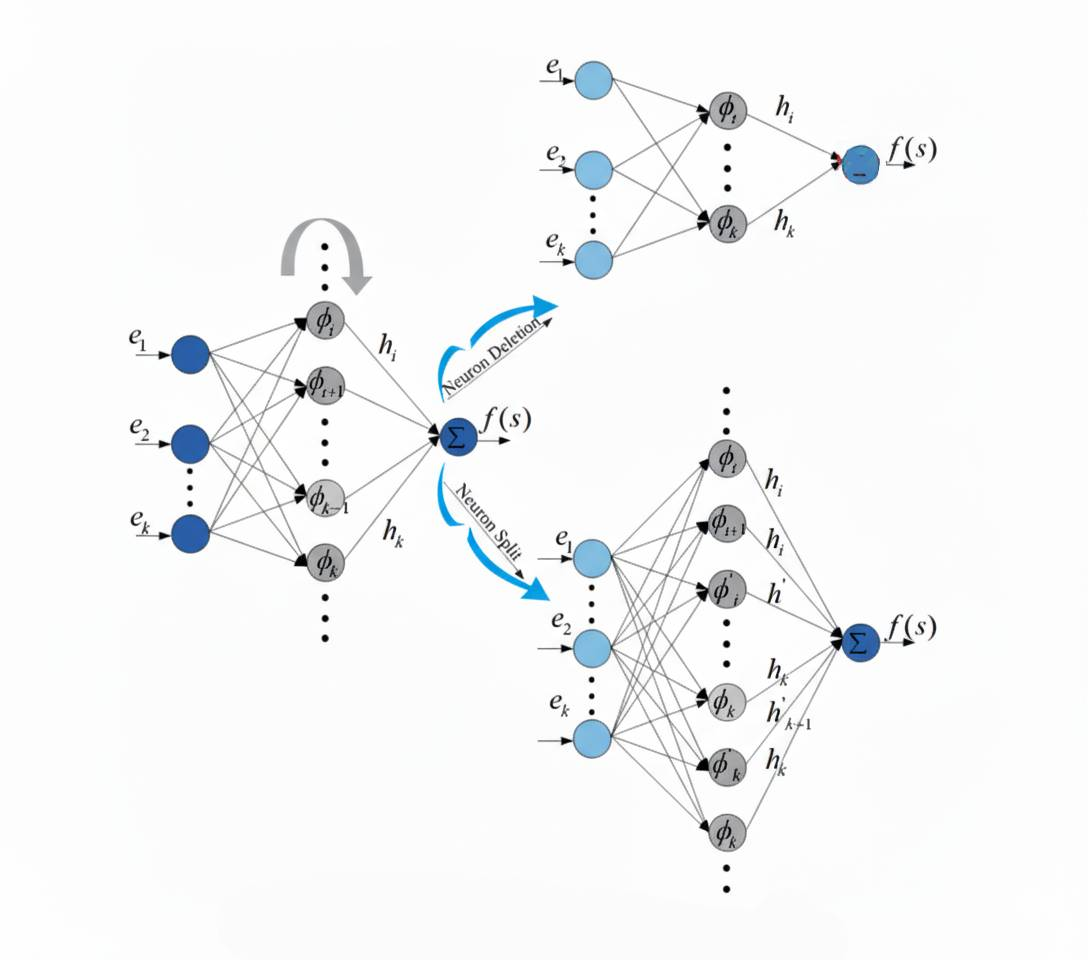
\includegraphics[width=0.8\textwidth]{Thesis_ICD/figure5/ssnn meca.jpg}
    \caption{The structure of the self-structuring neural network.}
    \label{fig:ssnn_structure}
\end{figure}

The weight vector is updated using an adaptive law:
\begin{equation}
    \dot{\hat{W}} = \Gamma s \Phi(Z) - \sigma \Gamma \hat{W}
    \label{eq:weight_update}
\end{equation}
where $\hat{W}$ is the estimate of $W$, and $\Gamma$ and $\sigma$ are positive design parameters.

\subsection{Distributed Formation Controller}
\label{subsec:formation_controller}

The formation controller is designed to ensure all follower UAVs maintain the desired separation vectors $h_i$ relative to the virtual leader $p_0$. The formation error for the $i$-th UAV is defined based on local neighborhood information:
\begin{equation}
    \epsilon_i = \sum_{j \in \mathcal{N}_i(t)} a_{ij}(t) \left( (p_i - h_i) - (p_j - h_j) \right) + b_i(t) (p_i - h_i - p_0)
    \label{eq:formation_error}
\end{equation}
where $\mathcal{N}_i(t)$ is the set of neighbors of UAV $i$ at time $t$. The control objective for the formation layer is to drive $\epsilon_i$ and its derivatives to zero. This is achieved by designing a distributed virtual control law that generates the desired position reference $p_{id}$ and its derivatives $\dot{p}_{id}, \ddot{p}_{id}$ for the position controller of each UAV.

\subsection{Position and Attitude Fault-Tolerant Control}
\label{subsec:position_attitude_control}

The position and attitude controllers for each UAV are designed using the ASNN-FTSMC framework. Let's consider the position subsystem for UAV $i$. The tracking errors are $e_{p1,i} = p_i - p_{id}$ and $e_{p2,i} = \dot{p}_i - \dot{p}_{id}$. The sliding surface is:
\begin{equation}
    s_{p,i} = e_{p2,i} + \alpha_{p1} |e_{p1,i}|^{\rho_{p1}} \text{sgn}(e_{p1,i}) + \alpha_{p2} |e_{p1,i}|^{\rho_{p2}} \text{sgn}(e_{p1,i}).
    \label{eq:position_sliding}
\end{equation}

The time derivative of the sliding surface is $\dot{s}_{p,i} = \ddot{p}_i - \ddot{p}_{id} + \dots$. Substituting the dynamics, we get:
\begin{equation}
    \dot{s}_{p,i} = f_{p,i} + g_{p,i} u_{p,i} + D_{p,i} - \ddot{p}_{id} + \alpha_{p1} \frac{d}{dt}(|e_{p1,i}|^{\rho_{p1}} \text{sgn}(e_{p1,i})) + \dots
    \label{eq:sliding_derivative}
\end{equation}
The fault-tolerant control law is designed to drive $s_{p,i}$ to zero in fixed time:
\begin{equation}
    u_{p,i} = g_{p,i}^{-1} \left( -f_{p,i} + \ddot{p}_{id} - \text{terms}(\dots) - k_{p1} s_{p,i} - k_{p2} |s_{p,i}|^{\gamma_p} \text{sgn}(s_{p,i}) - \hat{D}_{p,i} \right)
    \label{eq:position_control}
\end{equation}
where $k_{p1}, k_{p2} > 0$, $0 < \gamma_p < 1$, and $\hat{D}_{p,i} = \hat{W}_{p,i}^T \Phi(Z_{p,i})$ is the output of the ASNN estimator for the position subsystem. This control law calculates the desired total thrust $T_z$ and the desired roll and pitch angles, $\phi_d, \theta_d$.

A completely analogous ASNN-FTSMC is designed for the attitude subsystem to track the desired angles generated by the position controller, thereby computing the final control torques $\tau_\phi, \tau_\theta, \tau_\psi$.

\begin{theorem}
\label{thm:stability}
Consider the multi-UAV system with coaxial rotor dynamics subject to actuator and sensor faults, and a switching communication topology. Under the proposed distributed ASNN-FTSMC law, the formation tracking errors of each UAV are guaranteed to be practically fixed-time stable, converging to a small neighborhood of the origin in a fixed time that is independent of the initial conditions.
\end{theorem}

\begin{proof}[Sketch of Proof]
A composite Lyapunov function for the entire multi-agent system is constructed as $V = \sum_{i=1}^N V_i$, where $V_i$ is the Lyapunov function for the $i$-th UAV, defined as:
\begin{equation}
    V_i = \frac{1}{2}s_{p,i}^T s_{p,i} + \frac{1}{2}s_{\eta,i}^T s_{\eta,i} + \frac{1}{2}\text{Tr}(\tilde{W}_{p,i}^T \Gamma_{p,i}^{-1} \tilde{W}_{p,i}) + \frac{1}{2}\text{Tr}(\tilde{W}_{\eta,i}^T \Gamma_{\eta,i}^{-1} \tilde{W}_{\eta,i})
    \label{eq:lyapunov_function}
\end{equation}
where $\tilde{W} = W - \hat{W}$ are the neural network weight estimation errors. By taking the time derivative of $V$ and substituting the control laws and adaptation laws, it can be shown that $\dot{V}$ satisfies the condition for practical fixed-time stability from Lemma 2 in Chapter 2, i.e., $\dot{V} \le -\lambda_1 V^{\rho_1} - \lambda_2 V^{\rho_2} + h$. This guarantees that all sliding surfaces and estimation errors converge to a small residual set in a fixed time, ensuring the stability and performance of the formation.
\end{proof}
